\chapter{Navigation}
\label{cha:navigation}

For the navigation part the \acrshort{nav2} package was used, as described in \autoref{cha:techstack}. As mentioned, the only thing you need is to pass a \textbf{YAML configuration file} to \code{navigation\_bringup.py} script, and it will start up the nodes with the desired parameters set.

\section{\acrshort{nav2} nodes introduction}

This is a brief description of the nodes responsible for navigation, in order to get a better idea of the \textbf{workflow}. This is a summary of \code{README} files from their \textbf{GitHub} repository\cite{nav2github}. In \autoref{fig:nav2} you can see the \acrshort{nav2} architecture.

\bigskip

\begin{figure}[h]
    \centering
    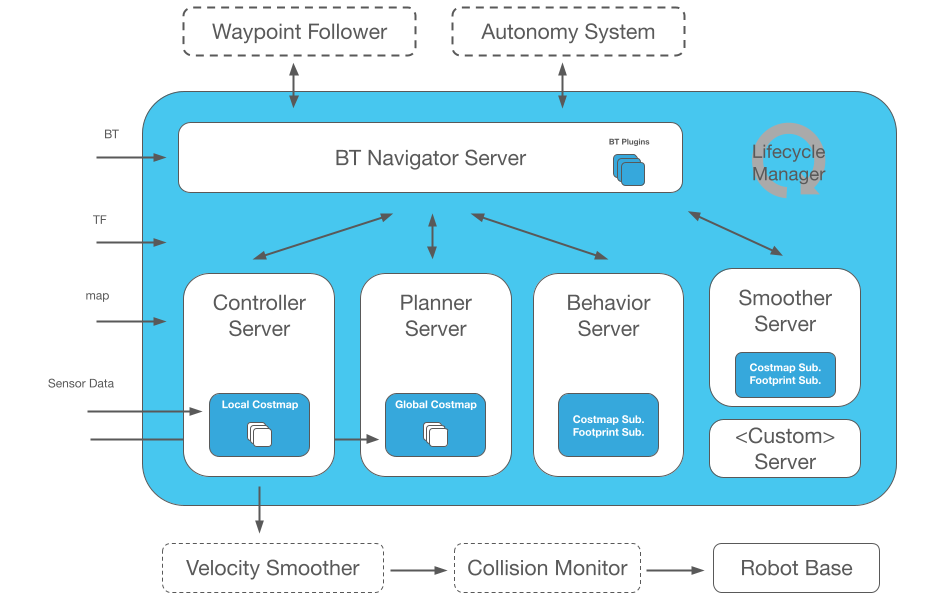
\includegraphics[width=0.8\textwidth]{images/nav2_architecture}
    \caption{Navigation package overview}
    \label{fig:nav2}
\end{figure}

\subsection{Map Server}

This package is used to provide \textbf{map} functionalities to \acrshort{ros}. Basically, it gives you the ability to \textbf{load} a map from a file and use it for \acrshort{amcl}, or \textbf{save} it after \acrshort{slam} has been run.

\subsection{\acrfull{amcl}}

\acrshort{amcl} is used to \textbf{locate} the robot on a known \textbf{map} using a 2D laser scanner \textbf{probabilistically}. First, once the map is loaded, the initial pose of the robot \textbf{must be set}\footnote{you can do it graphically with \acrshort{rviz}}: what is happening under the hood is publishing a \code{map} $\rightarrow$ \code{odom} transformation so that the \code{odom} $\rightarrow$ \code{base\_link} one leads to the \textbf{actual location} of the robot.

\subsection{\acrfull{slam}}

It is a collection of techniques used to \textbf{locate} and \textbf{map} the environment \textbf{simultaneously}, using 2D laser scans\cite{slam}. Once the map is fully built, you can save it to a file and pass it to the \textit{Map Server}.

\subsection{Recoveries Server}

It is responsible for performing simple controlled robot movements, such as going back, rotating or stopping when \textbf{recovery} is needed, like when the robot \textbf{hits} something.

\subsection{\acrfull{btnav}}

This makes use of \textbf{behavior trees} to define the actions to be performed when the robot is in a certain \textbf{state}: for example, when no problem is encountered, it will continue to navigate and reach the current goal, but when it hits something, the behavior tree will perform the recovery action.

\begin{figure}[h]
    \centering
    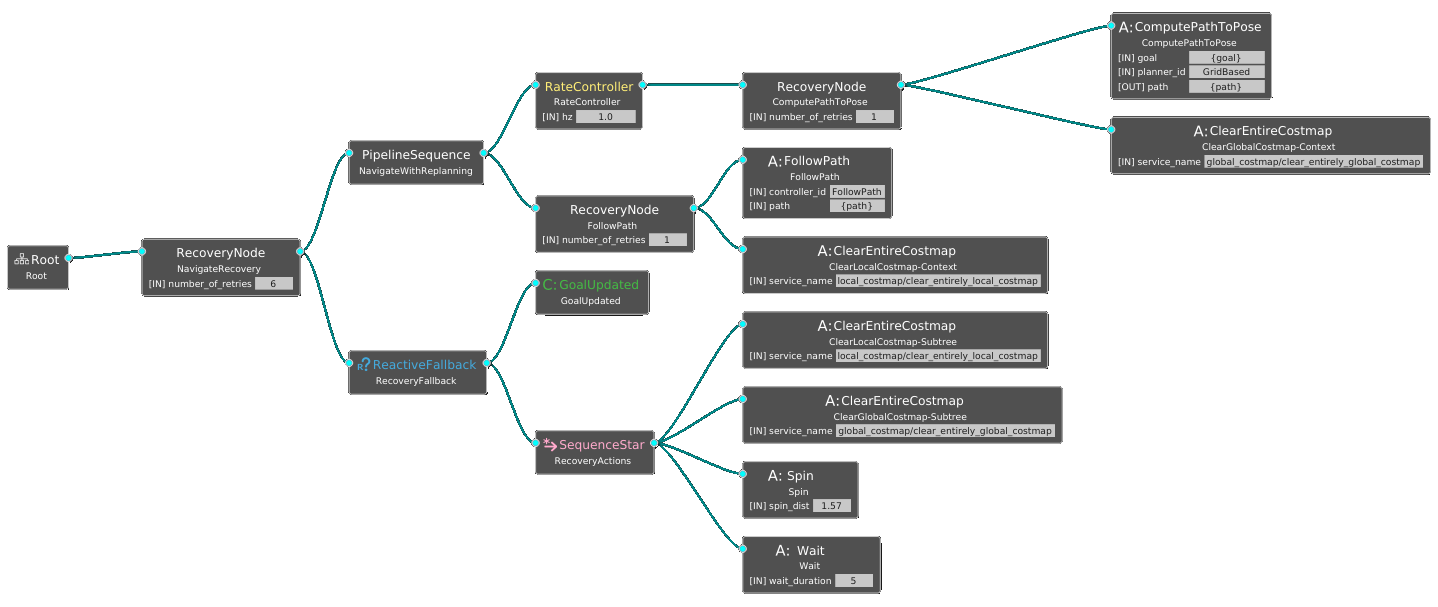
\includegraphics[width=\textwidth]{images/bt-alpha.png}
    \caption{Currently used behavior tree. Groot lets you visualize it, also in real-time\cite{groot}.}
\end{figure}

\subsection{Planner Server}

It implements behavior trees to \textbf{compute path to pose}; you can also choose which pathfinding algorithm you want to use.

\subsection{Controller Server}

It generates \textbf{command velocities} for the wheels using computed path from \textit{Planner Server} and send them to the robot.

% \subsection{Waypoint Follower} 

% Instead of just setting a single goal, it is possible to navigate a list of waypoints the robot has to pass through. When a waypoint is reached, some plugins can be attached in order to make the robot take a photo, wait for external command or simply wait. Currently, this feature has not been used in the project, because even if multiple rooms are requested to be visited, the planner will only generate subsequent tasks, passing them one by one, after the previous one has been completed.

\subsection{Lifecycle Manager}

All the previous nodes interface with \textbf{Lifecycle Manager}, which brings \acrshort{ros}2 \textbf{managed nodes}\footnote{\textit{A managed life cycle for nodes allows greater control over the state of ROS system. [...] a managed node presents a known interface, executes according to a known life cycle state machine, and otherwise can be considered a black box}\cite{lifecycle}} concept to the navigation stack: in such a manner, before nodes begin their execution, it \textbf{checks} if all have been \textbf{launched correctly} and are ready to start, to avoid unexpected behaviors.

\begin{figure}[h]
    \centering
    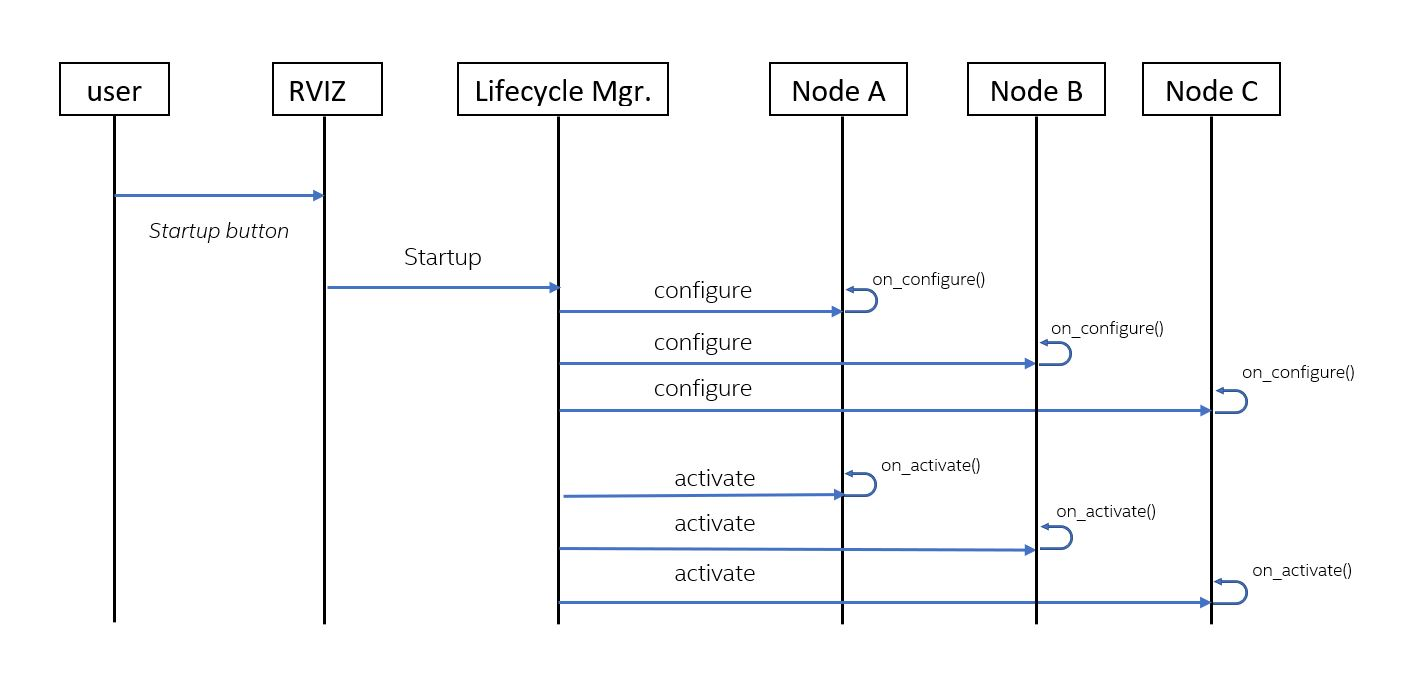
\includegraphics[width=0.9\textwidth]{images/uml_lifecycle_manager}
    \caption{Sequence of service calls when startup is requested}
\end{figure}

\section{Navigation setup}

\begin{wrapfigure}[15]{r}{0.35\textwidth}
    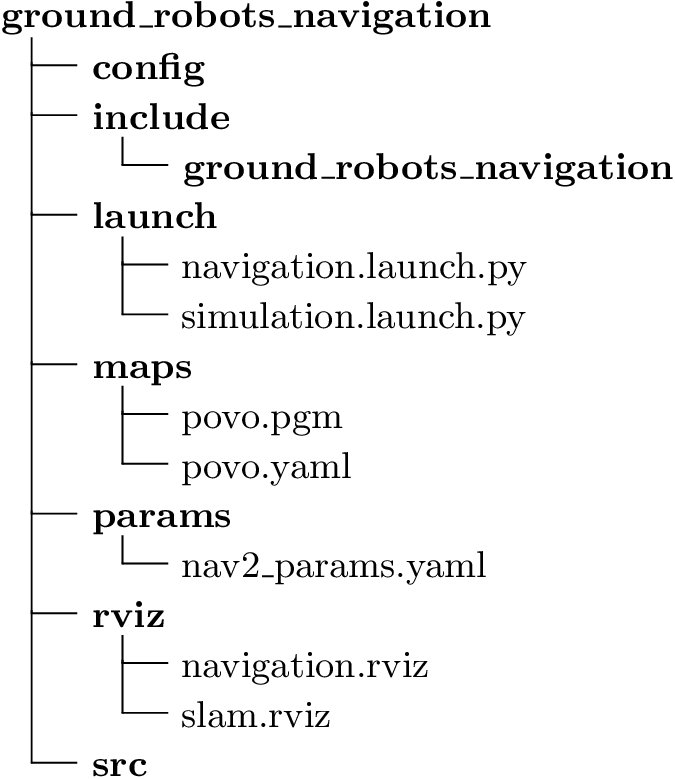
\includegraphics[width=0.35\textwidth]{images/nav_folder}
    \caption{Navigation folder}
\end{wrapfigure}

Regardless of whether the robot is real or simulated, there is always a \code{scan}, \code{odom} and \code{cmd\_vel} topic and a \code{map}, \code{odom} and \code{base\_link}\footnote{All the other links of the robot are connected to this, the root one} frame.

When it comes to setting up navigation properties, the most important is \code{costmap}, which is divided into a global and a local one. Here follows a brief description:
\begin{itemize}
    \item \textbf{Global}: it is created on the basis of the map provided, saved from \acrshort{slam}, to create the \textbf{general area} where the robot can and cannot move; it also contains information on how far the robot should keep \textbf{from the walls}; used for planning paths.
    \item \textbf{Local}: it uses lidar data to create the \textbf{actual zones} where the robot can and cannot move; in this case, the data received is dynamic, and it is used to adapt the robot's behavior to changes in the environment (e.g. unforeseen obstacles and therefore \textbf{avoids} them).
\end{itemize}

To automatically display the robot and environment on \acrshort{rviz}, a configuration file has been created: it keeps track of the map, costmaps, robot shape (described in the \acrshort{urdf} file as discussed in \autoref{sub:robot}), lidar and odom frame. 

The map currently in use was created using \acrshort{slam}, and since it is quite hard to graphically control the robot with \acrshort{rviz} when doing so\footnote{The map is currently being generated and it may happen that the robot hits a wall when specifying a goal position, because it is not already aware of rooms boundaries}, another way must be found: the solution is the \code{joy} driver package, which makes an \textbf{Xbox controller} capable of setting wheels velocity over \code{cmd\_vel} topic (via \textbf{Bluetooth}).

Everything is then put together inside a \textbf{launch file} (a custom Python script); inside it are described which \textbf{nodes} should be started, and also the \textbf{parameters} that can be passed from command line (overriding their default value). For example, if you want to start a simulation, you need to set the \code{use\_simulator} parameter to \textit{true} (normally it is \textit{false}); the same goes for \textbf{disabling} the Gazebo \acrfull{gui}: you can set \textbf{headless} to \textit{true}. These parameters, as shown above, can be used to perform \textbf{conditional checks}, in order to decide whether a node should be started or not.